\documentclass[compress, containsverbatim,mathserif, xcolor=dvipsnames, unicode]{beamer}


%tema
\usetheme{Antibes}
%\usecolortheme[named=Maroon]{structure}
\usecolortheme{default}





% zbog srpskog
\usepackage[serbian]{babel}
\usepackage[utf8]{inputenc}
\usepackage[T2A]{fontenc}

% za matematiku
\usepackage{amsmath}
\usepackage{amssymb}
\usepackage{fontawesome5}

\usepackage{xcolor}

\newtheorem{primer}{Primer}[section]

\title{Informacioni sistem auto škole}
\author{Emilija Stošić, Mirko Ilić, Tamara Stojković}
\institute{Informacioni sistemi \\ Matematički fakultet \\ Univerzitet u Beogradu}
\date{
	\footnotesize{Beograd, decembar 2022.}	
}

\begin{document}

\begin{frame}
\titlepage

\begin{figure}[h!]
    \centering
    \begin{flushleft}
    
\includegraphics[width=15mm]{logo.png}
    \end{flushleft}
\end{figure}
\end{frame}

\begin{frame}{Sadržaj}
\tableofcontents
\end{frame}

\section{Uvod}
\begin{frame}{Uvod}
\vspace{\baselineskip}
\begin{itemize}
	\item Informacioni sistem auto škole 
    \begin{itemize}
        \item prati kandidata od upisa do izdavanja dozvole
        \item uključuje i  praćenje zaposlenih kadrova
    \end{itemize}
    \item Zaposleni imaju određene uloge u procesu evidencije i obuke kanidata
    \item Primarni cilj - da se unapredi način funkcionisanja postojećih sistema za auto školu
    \item Uvodi se veći broj zaposlenih, online formulari, ankete

\end{itemize}
\end{frame}

\section{Analiza sistema}
\subsection{Akteri}
\begin{frame}{Akteri}
        \begin{figure}[h!]
        \begin{center}
          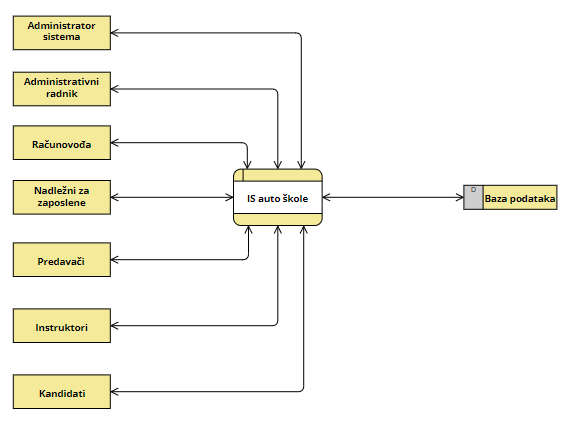
\includegraphics[scale = 0.5]{dijagram_konteksta.png}
        \end{center}
       \caption{Dijagram konteksta}
    \end{figure}   
\end{frame}

\section{Slučajevi upotrebe}
\begin{frame}{Slučajevi upotrebe}
\vspace{\baselineskip}
\begin{itemize}
	\item Razlikujemo 5 glavnih slučajeva upotrebe:
    \begin{itemize}
        \item Podnošenje zahteva za prijavu
        \item Teorijska nastava
        \item Praktična nastava
        \item Vođenje evidencije
        \item Vođenje finansija
    \end{itemize}
    \item Svaki od njih je podeljen na više manjih slučajeva
    
\end{itemize}
\end{frame}


\subsection{Podnošenje zahteva za prijavu}
\begin{frame}{Podnošenje zahteva za prijavu}
        \begin{figure}[h!]
        \begin{center}
          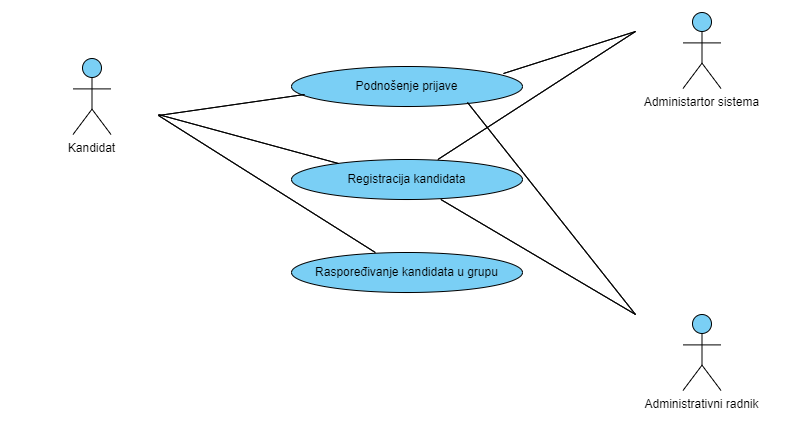
\includegraphics[scale = 0.5]{podnosenje_zahteva_za_prijavu.png}
        \end{center}
       \caption{Dijagram slučaja upotrebe}
    \end{figure}   
\end{frame}

\begin{frame}{Dijagram stanja}
        \begin{figure}[h!]
        \begin{center}
          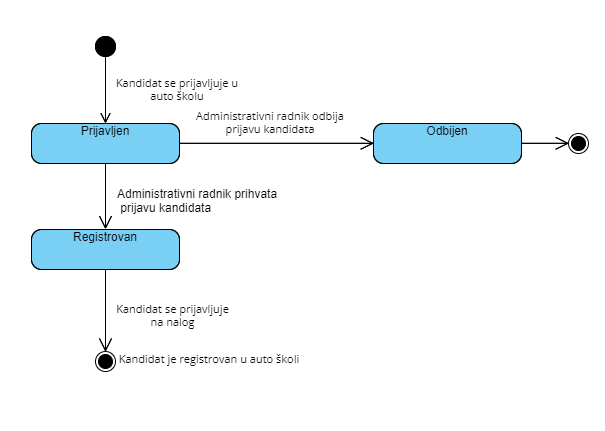
\includegraphics[scale = 0.5]{dijagram_stanja_registracija.png}
        \end{center}
       \caption{Dijagram stanja - podnošenje zahteva za prijavu}
    \end{figure}   
\end{frame}


\subsection{Teorijska nastava}
\begin{frame}{Teorijska nastava}
        \begin{figure}[h!]
        \begin{center}
          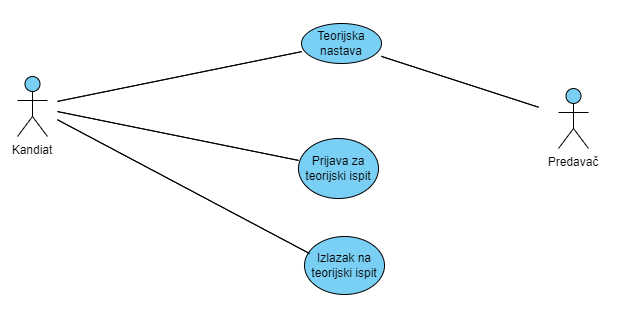
\includegraphics[scale = 0.6]{diagram teorijska nastava.png}
        \end{center}
       \caption{Dijagram slučaja upotrebe}
    \end{figure}   
\end{frame}



\subsection{Praktična nastava}
\begin{frame}{Praktična nastava}
        \begin{figure}[h!]
        \begin{center}
          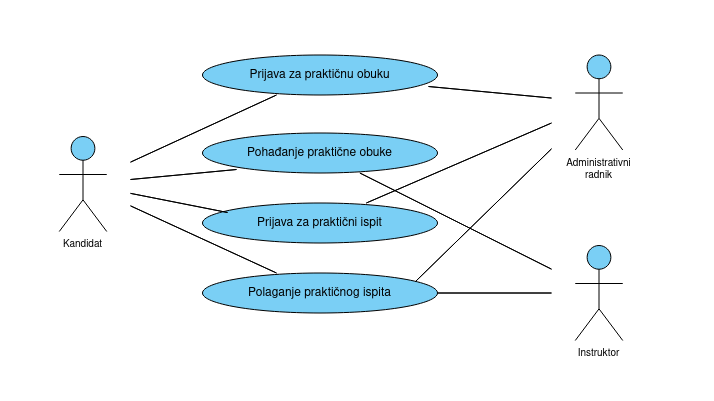
\includegraphics[scale = 0.4]{prakticna_obuka.png}
        \end{center}
       \caption{Dijagram slučaja upotrebe}
    \end{figure}   
\end{frame}


%\begin{frame}{Dijagram stanja kandidata}
 %   \begin{figure}[h!]
    %\begin{center}
    %  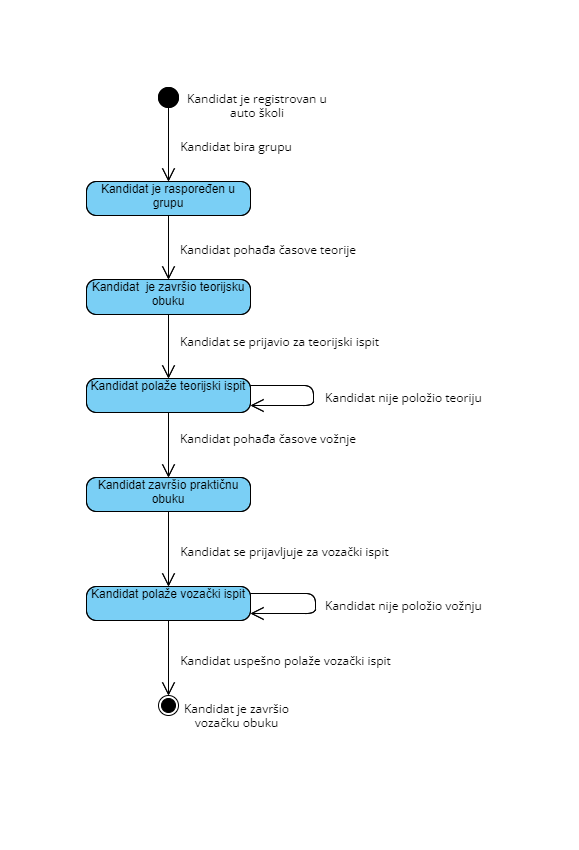
\includegraphics[scale = 0.35]{dijagram_stanja_kandidata.png}
    %\end{center}
   %\caption{Dijagram stanja  kandidata u celom procesu obuke}
%\end{figure}   
%\end{frame}

\subsection{Vođenje evidencije}
\begin{frame}{Vođenje evidencije}
        \begin{figure}[h!]
        \begin{center}
          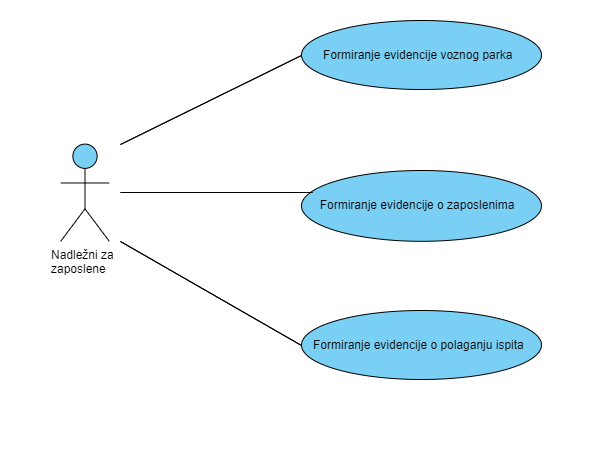
\includegraphics[scale = 0.5]{evidencija.png}
        \end{center}
       \caption{Dijagram slučaja upotrebe}
    \end{figure}   
\end{frame}

\subsection{Vođenje finansija}
\begin{frame}{Vođenje finansija}
        \begin{figure}[h!]
        \begin{center}
          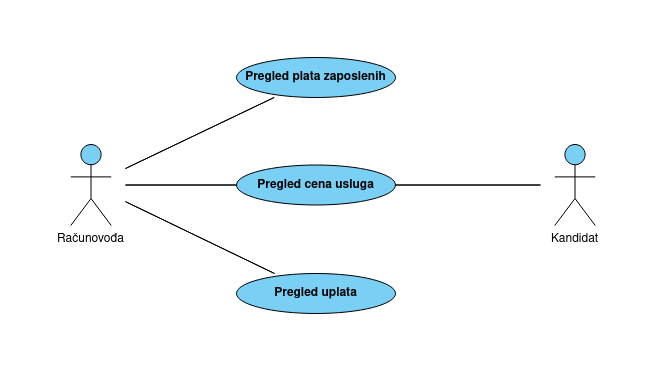
\includegraphics[scale = 0.45]{vodjenje_finansija.png}
        \end{center}
       \caption{Dijagram slučaja upotrebe}
    \end{figure}   
\end{frame}

\section{Opis baze podataka}
\begin{frame}{Opis baze podataka}
\vspace{\baselineskip}
\begin{itemize}
	\item U bazi su predstavljeni podaci podeljeni u 4 grupe podataka:
    \begin{itemize}
        \item Podaci o osoblju i kandidatu
        \item Podaci o ispitu
        \item Podaci o nastavi
        \item Ostali podaci
    \end{itemize}
    \item Baza je predstavljena u radu dijagramom klasa
   

\end{itemize}
\end{frame}


\section{Arhitektura sistema}
\begin{frame}{Arhitektura sistema}
\vspace{\baselineskip}
\begin{itemize}
	\item Karakteristike arhitekture sistema:
    \begin{itemize}
        \item Tip aplikacije: Veb aplikacija
        \item Strategije isporučivanja: Jedan serverski i više klijentskih računara
        \item Tehnologije: Node.js, Angular,MongoDB baza podataka
    \end{itemize}
   

\end{itemize}
\end{frame}


\section{Korisnički interfejs}
\begin{frame}{Korisnički interfejs}
\vspace{\baselineskip}

	Predstavljeni su sledeći delovi aplikacije:
    \begin{itemize}
        \item Podnošenje prijave u auto školu
        \item Prijavljivanje kandidata na nalog
        \item Profil kandidata
        \item Izbor grupe
        \item Prijavljivanje ispita
        \item Profil računovođe
        \item Pregled uplata
        \item Profil nadležni za zaposlene
        \item Evidencija vozila
        \item Profil predavača i instruktora
   
    \end{itemize}
\end{frame}


\begin{frame}{Prijava ispita}
        \begin{figure}[h!]
        \begin{center}
          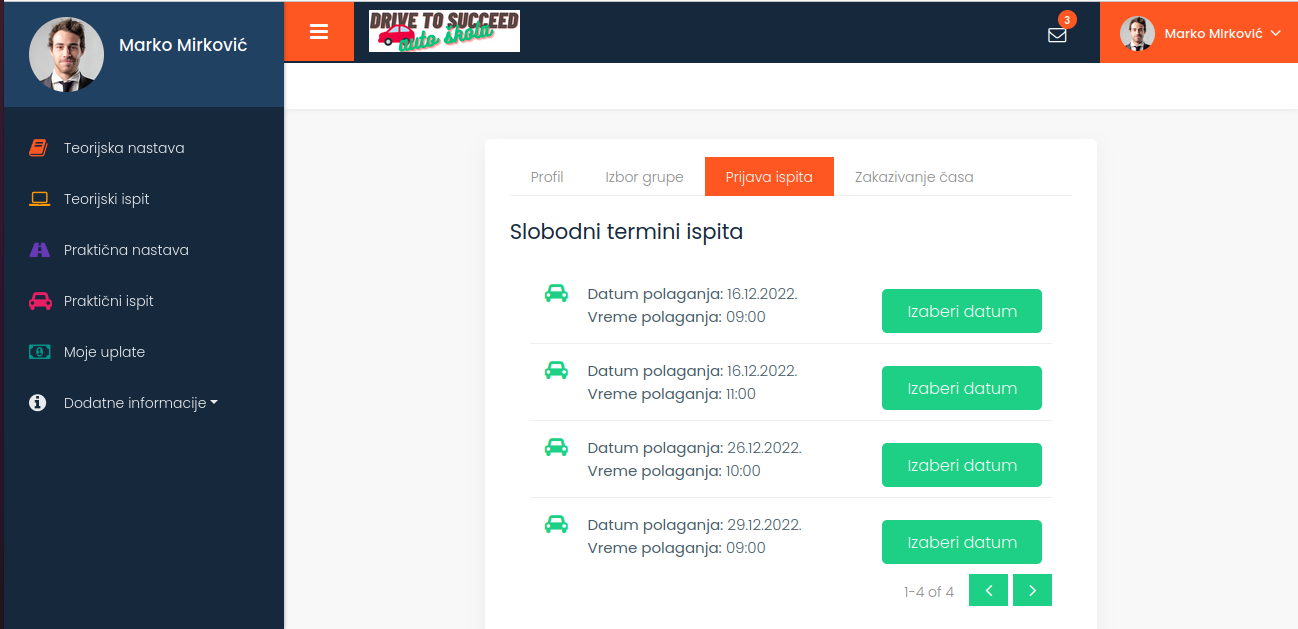
\includegraphics[scale = 0.25]{UI_prijava_ispita.png}
        \end{center}
       \caption{Prijava ispita  }
    \end{figure}   
\end{frame}


\begin{frame}{Evidencija vozila}
        \begin{figure}[h!]
        \begin{center}
          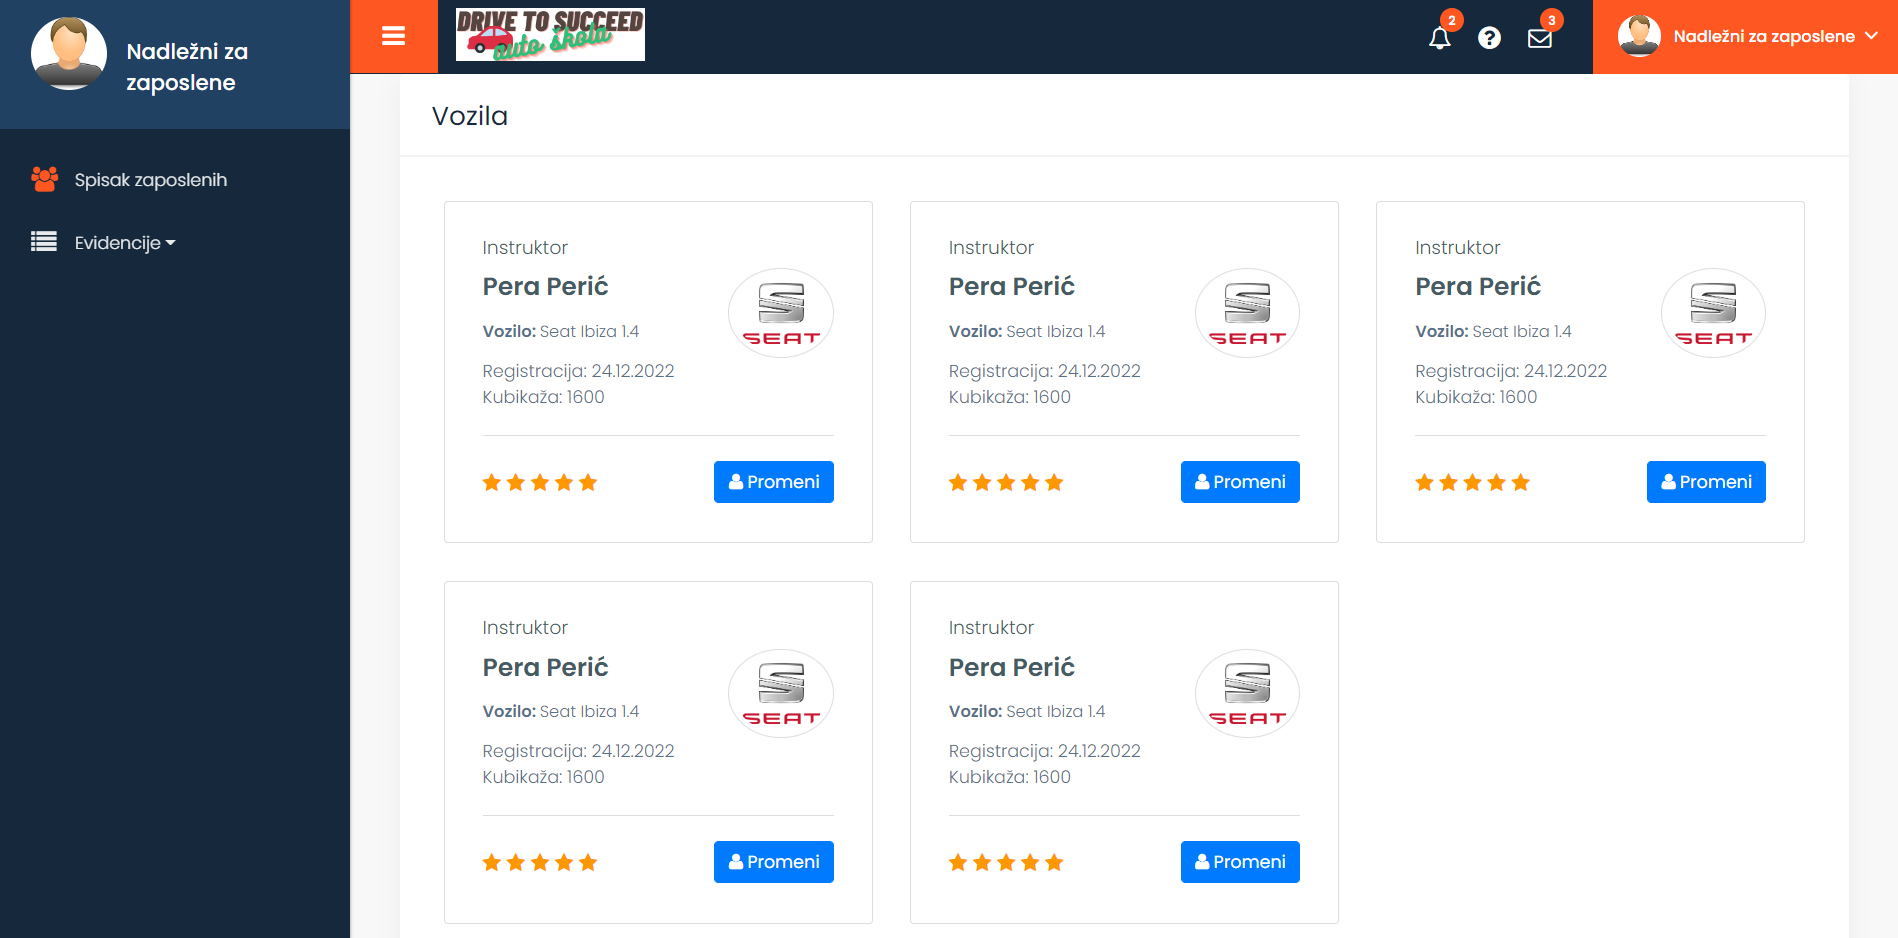
\includegraphics[scale = 0.27]{UI_Nadlezni_za_zaposlene_vozila.png}
        \end{center}
       \caption{Lista vozila }
    \end{figure}   
\end{frame}

\begin{frame}{Pregled uplata}
        \begin{figure}[h!]
        \begin{center}
          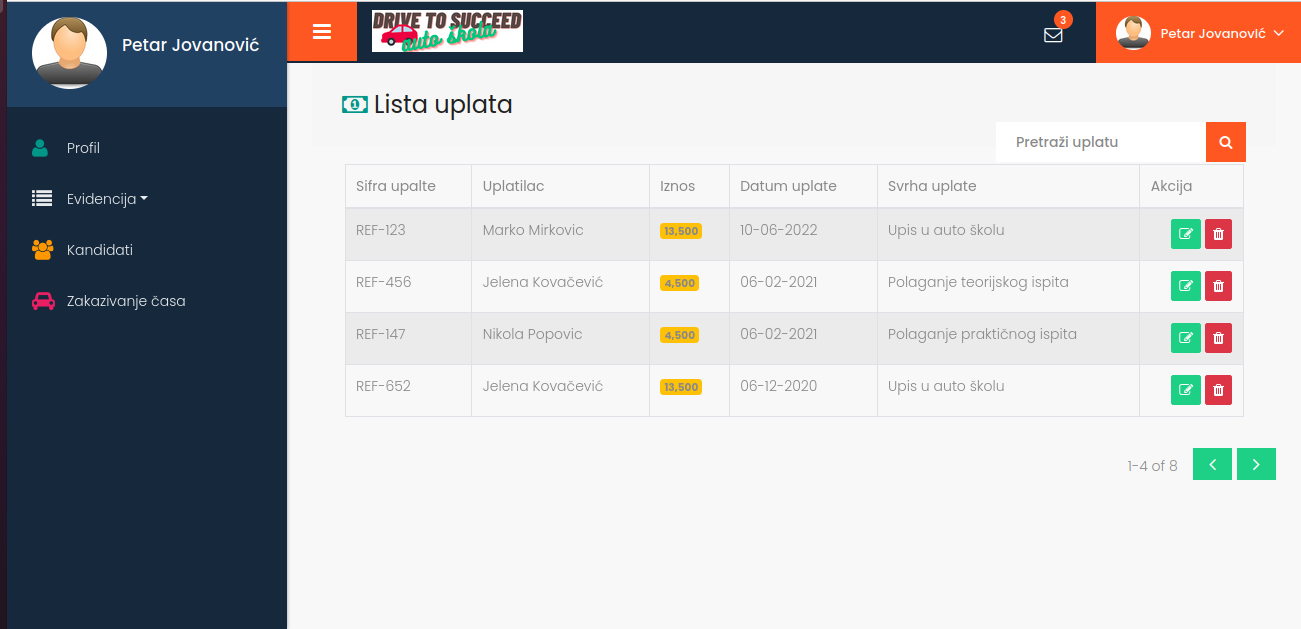
\includegraphics[scale = 0.25]{UI_lista_uplata.png}
        \end{center}
       \caption{Lista uplata kandidata }
    \end{figure}   
\end{frame}


\begin{frame}{}
        \begin{center}
        \Huge HVALA NA PAŽNJI!
        \end{center}



\end{frame}















\end{document}

    
